\documentclass[12pt]{article}

\addtolength{\textwidth}{.8in}
\addtolength{\hoffset}{-.4in}
\addtolength{\textheight}{1in}
\addtolength{\voffset}{-1in}

\usepackage{amsmath}
\usepackage{graphicx}
\usepackage{upquote} % to convert funny quotes to straight quotes
\usepackage{amsfonts}
\usepackage{paralist}
\setlength{\parindent}{15pt}

\renewcommand*{\thefootnote}{\fnsymbol{footnote}}

\begin{document}

\begin{center}
\begin{Large}
DATA 219 Notes -- Feb. 6, 2018
\end{Large}
\end{center}

\section{``Hierarchical" vs. ``flat" data}

As we learned last week, the JSON file format can be seen as essentially a
textual representation of an arbitrarily nested Python object. This object can
be a list or a dictionary, and have embedded lists and dictionaries to any
arbitrary level of nesting. Here's an example:

\begin{Verbatim}[fontsize=\small,samepage=true,frame=none]
[{"prefix": "DATA", "num": 219, "creds": 3, "instructor": "Davies",
"meetings": [{"time": {"day": "TR", "time": "2pm"}, "location": {"bldg":
"Trinkle", "room": "B6"}}], "roster": [{"first": "Lady", "last": "Gaga",
"email": "lgaga@umw.edu"}, {"first": "The", "last": "Rock", "email":
"trock@umw.edu"}, ...
\end{Verbatim}

When you disentangle this, you'll realize that what you have is:

\vspace{.2in}

\large
\noindent A list, each element of which is:\\
$\bullet$ a dictionary, with key/value pairs:
        \begin{compactenum}
        \item \texttt{prefix}: a string
        \item \texttt{num}: an int
        \item \texttt{creds}: an int
        \item \texttt{instructor}: a string
        \item \texttt{meetings}: a list, each element of which is:
            \begin{compactitem}
            \item a dictionary, with key/value pairs:
                \begin{compactenum}
                \item \texttt{time}: a dictionary, with key/value pairs:
                    \begin{compactenum}
                    \item \texttt{day}: a string
                    \item \texttt{time}: a string
                    \end{compactenum}
                \item \texttt{location}: a dictionary, with key/value pairs:
                    \begin{compactenum}
                    \item \texttt{bldg}: a string
                    \item \texttt{room}: a string
                    \end{compactenum}
                \end{compactenum}
            \end{compactitem}
        \item \texttt{roster}: a list, each element of which is:
            \begin{compactitem}
            \item a dictionary, with key/value pairs:
                \begin{compactenum}
                \item \texttt{first}: a string
                \item \texttt{last}: a string
                \item \texttt{email}: a string
                \end{compactenum}
            \end{compactitem}
        \item ...and possibly other stuff...
        \end{compactenum}

\normalsize

\pagebreak

This kind of structure is called \textbf{hierarchical} data. This is in
contrast to so-called \textbf{flat} data, like a CSV:

\begin{Verbatim}[fontsize=\small,samepage=true,frame=none]
Prefix,Num,Instructor,Creds,Bldg,Room,Day,Time
DATA,219,Davies,3,Trinkle,B6,TR,2pm
ENGL,286,Rigsby,3,Combs,112,MWF,11am
CPSC,305,Finlayson,4,Trinkle,B52,MWF,8am
\end{Verbatim}

It should be clear that hierarchical data is intrinsically more expressive
than flat data. Rather than each data record being a strict, identical-length
sequence of values, the whole nested structure communicates order and
relationships between subcomponents, like an outline.

It's not even always possible, let alone straightforward, to convert from a
hierarchical format to a flat format. Consider the JSON file above: it permits
any number of \texttt{meetings} for a single course, each of which has
embedded structure. In this case, the structure for each meeting is regular,
since it's apparently composed of a fixed number of fields with unique names.
(This won't always be the case, and if it's not, we would \textit{lose
information} in collapsing it to a flat format.) Even so, though, it's not
clear what to do with the multiple meeting times/locations for a course. Do we
make each \texttt{Bldg/Room/Day/Time} group into its own set of headings in
the flat format? This brings with it its own problems, such as:

\begin{compactenum}
\item How do we associate each group of buildings/rooms/days/times together,
since they're now all individual top-level fields? (Naming conventions seem
like the only solution, and it's awkward.)
\item How do we know the maximum number of such meetings, so as to specify the
width of the table?
\item What do we do for rows which don't have the maximum number of meetings?
Leave the others blank?
\item How do we perform standard queries like ``find all courses that have at
least one meeting in Trinkle?" (We have to split this up into an awkward query
that separately queries each of the columns and unions the answer.)
\end{compactenum}

There are better ways to organize such data, such as the \textbf{relational
model} that has been ubiquitous in database schema design since Ted Codd
invented it in the 1960's. It allows us to ``normalize" such data sets and
represent them in multiple, interrelated tables. We'll take a look at this
when we look at SQLite later in the course. Some irregular structures defy
even the relational model, however, which is why some newer database paradigms
(like NoSQL databases) have been developed to get around its limitations.

One big reality to grasp, however, is that at this point in time,
\textit{almost all machine learning algorithms are based on a \textbf{flat}
data structure}. There are some quite advanced, cutting-edge exceptions to
this, but really the field of mining hierarchical (and other non-flat) data
formats is still in its infancy. Lots of opportunity to make a name for
yourself here!

\section{Locally Weighted Regression (LOESS/LOWESS)}

A common exploratory technique for bivariate, numerical data involves finding
a smooth curve to approximate a noisy data set. The structure of the data --
and whether there even is a relationship between the two variables -- may be
more easily visible from such a curve than from a raw splattering of points.

\subsection{``Parametric" approximations}

In your stats class, you probably learned how to compute the best-fit line
to a set of bivariate numerical data points, where ``best fit" was taken in a
``least squares" sense (\textit{i.e.}, the line that minimizes the sum of the
squared deviations of the line from the actual data points). It will not
surprise you that it's easy to do this in Python as well, to wit:

\line(1,0){400}
\begin{Verbatim}[fontsize=\small,samepage=true,frame=none]
# Create some random x points and some crazy, noisy y function based on them.
x = np.random.uniform(0,100,100)
x.sort()
y = 4*x - .2 * x**2 + np.random.normal(0,120,100)

# Get the slope and intercept of the best-fit line.
m, b = np.polyfit(x, y, 1)

# Heck, while we're at it, let's find the best-fit quadratic, too.
a1, a2, a3 = np.polyfit(x, y, 2)

# Plot the points and the approximations.
plt.scatter(x,y)
plt.plot(x, m*x + b,color="green")
plt.plot(x, a1*x**2 + a2*x + a3,color="purple")
\end{Verbatim}
\quad \line(1,0){400}
 
\begin{center}
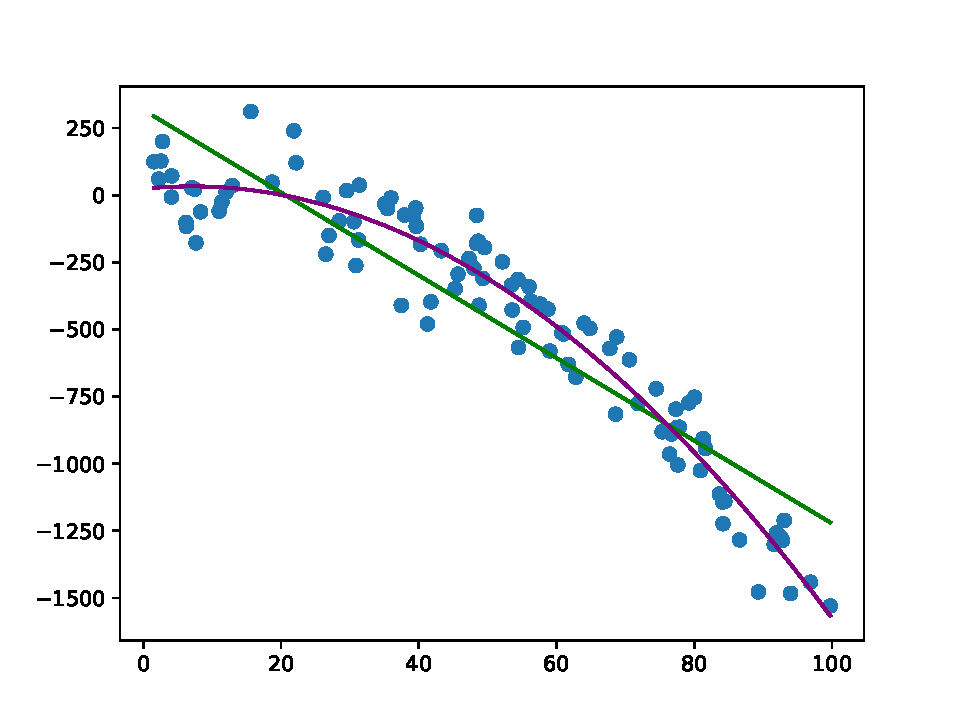
\includegraphics[width=0.8\textwidth]{bestfit.pdf}
\end{center}

(Note that we had to \texttt{.sort()} the $x$ points since we were going to
draw line plots based on them, and you get crazy zig-zags if you don't sort
your $x$ values first.)

These approximations are called \textit{parametric} models because they're
based on (global) parameters: a slope and an intercept, say, or three
coefficients in the case of the quadratic. In each case, we assume the data
fit an overall particular ``functional form" (like a line, or a quadratic) and
say, ``given that we feel like these data are `really' a line, what parameters
that describe a line would give us the best line?"

\subsection{LOESS: a ``Non-parametric" approximation}

LOESS accomplishes something similar -- capturing the overall trend of a messy
set of data -- but what distinguishes it from a best-fit line is that it
operates \textit{locally} rather than globally. When you crunch the numbers to
find the best-fit least-squares line to a data set, you're asking, ``what
values of slope and intercept for a \textit{single} line across the
\textit{entire} data set will give me the lowest \textit{overall} deviation
from the points?" (The same is true for a best-fit quadratic, cubic,
\textit{etc.}) In other words, you're attempting to fit a single model over
the entire range of data, and penalizing inaccuracies equally everywhere.

By contrast, the LOESS technique approximates the data \textit{locally}. This
means that it weights the data points in such a way that points close to the
location of interest contribute more strongly than do data points farther
away. It does this by fitting a linear (or polynomial) regression to each $x$
point of interest, but using a \textit{weighted} contribution from the nearby
points.

Here's how it works. We start with a bunch of $(x,y)$ points, and we want to
compute a ``locally smoothed" $y$ for every one of the $x$'s. 

First, we have a parameter $\alpha$ that specifies \textit{what fraction of
the data} to take into account (at all) for each estimate. This can be any
value from 0 to 1. You might guess that the smaller it is, the more wiggly
it'll allow our smoothed estimate to be, since we'll be considering only a
small number of points. This is true, as we'll see.

Then, once we've fixed $\alpha$, we're going to find a bunch of best-fit,
least-squares lines, one at each $x$ value. This is just like in regular old
linear regression. The catch is that instead of minimizing the \textit{sum} of
squared errors, we're going to minimize the \textbf{weighted} sum. And we'll
place a greater weight on the errors for $x$ points close to the one we're
evaluating. This will have the effect of allowing the curve to bend closely to
our actual data points while ignoring stuff that's far away.

In equations, the best-fit line approach finds an $m$ and $b$ that minimize
the overall sum of squared deviations (or ``residual sum of squares"):

\begin{align*}
RSS = \sum_i (y_i - (mx_i + b))^2
\end{align*}

But with LOESS, we calculate this separately for every $x$ point, and we
weight this with a \textit{weight function} $w$:

\begin{align*}
RSS(x) = \sum_i w(x-x_i) \cdot (y_i - (mx_i + b))^2
\end{align*}

Note how the weight function is given the distance between the $x$ value of
interest and the locations of the actual data points. Since we want to weight
close-by points more heavily, the $w$ should be higher for values closer to 
0.\footnote{You might notice that the weight function is much like the
\textit{kernel} for KDEs: in fact, it really is basically a kernel. Thus we
can use a Gaussian for it, just like we did for KDEs, although it's more
common with LOESS to use the so-called ``tri-cube" kernel: $w(\Delta x) = (1 -
|\Delta x|^3)^3$ for $|x|<1$ (and 0 otherwise).}

This is non-parametric because when we're done, if somebody asked, ``hey, I
like your LOESS curve -- what parameters did you use for it?" the answer would
be ``uh...there really aren't any parameters." The curve is a messy
combination of a bunch of different shifting approximations that we calculated
as we went through the whole data set. We didn't choose parameters to plug
into a particular model; in fact, we didn't really \textit{have} a model.

Like KDEs, this technique wasn't computationally possible until the age of
computers. Hence it's one of the newer kids on the block. Here's how to do it
in Python:

\vspace{.8in}
\pagebreak
\line(1,0){400}
\begin{Verbatim}[fontsize=\small,samepage=true,frame=none]
import statsmodels.nonparametric.smoothers_lowess

lowess = statsmodels.nonparametric.smoothers_lowess.lowess(y,x,frac=1/3)
plt.plot(lowess[:,0],lowess[:,1],color="red")
\end{Verbatim}
\quad \line(1,0){400}

\vspace{.2in}

The ``\texttt{frac}" parameter is our $\alpha$. Here's the match to the
previous data set for two different values of $\alpha$:

\begin{center}
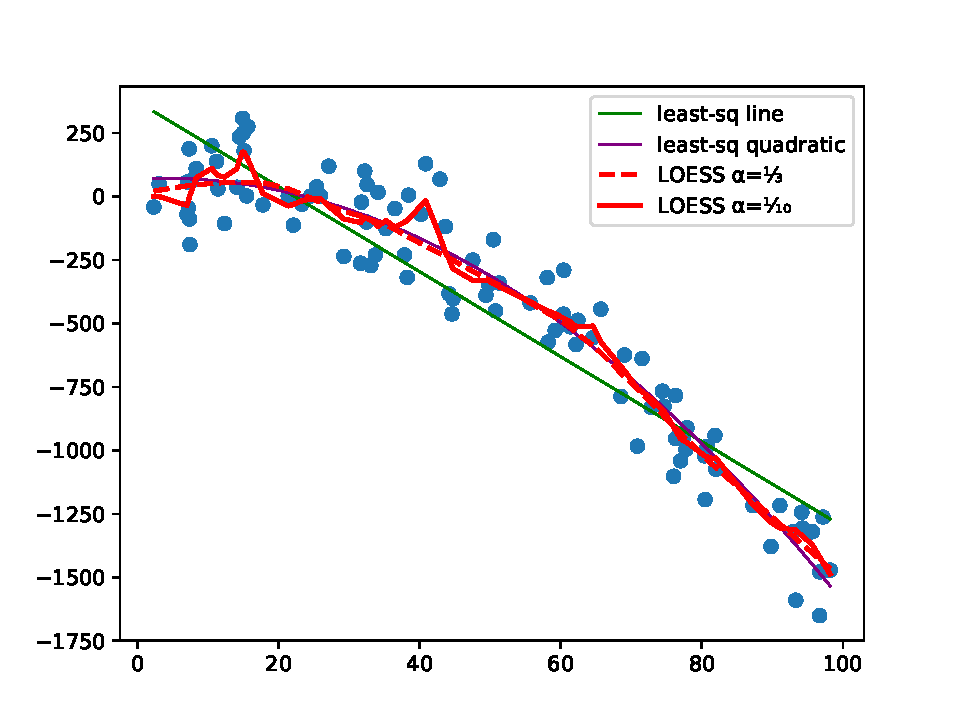
\includegraphics[width=0.8\textwidth]{lowess.pdf}
\end{center}

Notice how $\alpha = \frac{1}{3}$ gives a much smoother line than $\alpha =
\frac{1}{10}$, since it is using more points to do the smoothing. In fact, the
former is quite close to the best-fit quadratic in this case. This is a
manifestation of the classic ``bias-variance tradeoff" we'll talk about later
in the semester.

And finally, a data set where neither the line nor the quadratic are even in
the ballpark, but where LOESS does quite well:

\begin{center}
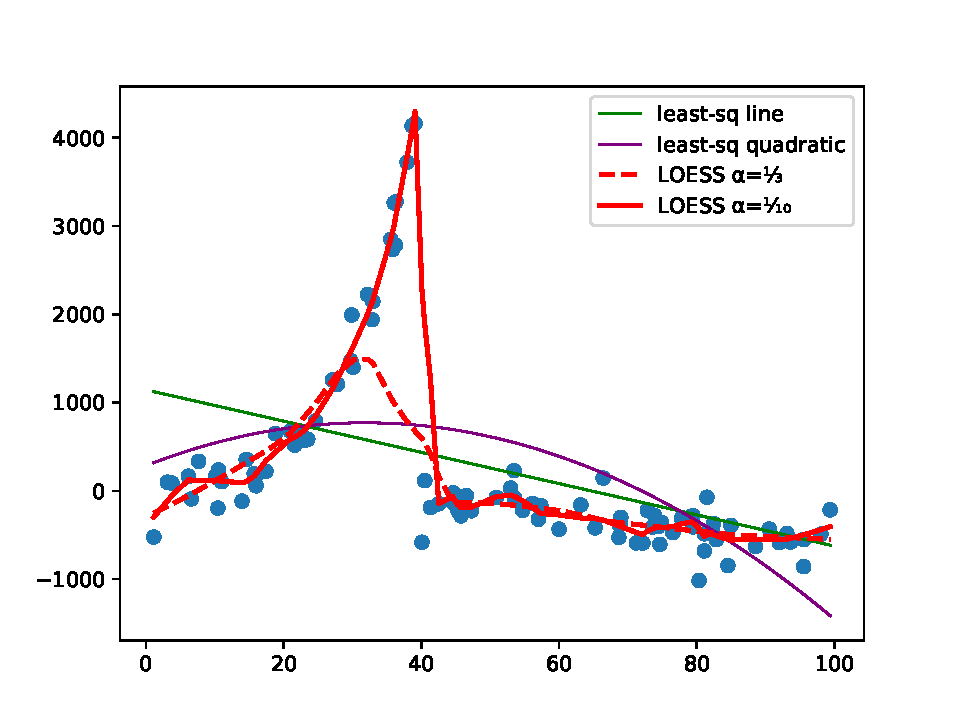
\includegraphics[width=0.8\textwidth]{lowess_better.pdf}
\end{center}

In general, LOESS is a better \textit{exploratory} technique than best-fit
parametric curves are. This is true for a couple of reasons:

\begin{compactitem}

\item When exploring a data set, you're looking for patterns that stick out,
and you want to let the data speak for itself. You're not coming to the data
with a pre-established model choice and wanting to fit it. LOESS lets you be
model-agnostic and yet see the forest instead of just trees.

\item LOESS (and non-parametric methods in general) are ``robust," meaning
they aren't as adversely affected by outliers. Consider fitting a
least-squares line to a set of data, and then introducing a couple of
high-leverage outliers near one of the far ends. This is going to force your
global-error-minimizing best-fit line to swing radically away from the bulk of
the data (which it may describe fairly adequately) in order to try and reach
those outliers. Clearly this isn't a good fit for the data! LOESS, however,
will only ``reach" for those outliers in the $x$ range when it gets near those
outliers.

\end{compactitem}

\vspace{.1in}

By the way, although we fit a \textit{linear} function to each local point, we
could fit a quadratic, cubic, or anything else. Here's something to think
about: if we replaced the linear ``$mx+b$" function with just a constant
``$b$", then LOESS becomes simply a weighted moving average. Oooo, deep.

\vspace{.1in}

Finally, remember to play with the $\alpha$ parameter just as you played with
the kernel width and bin size in other exploratory techniques. Remember:
changing this will give you different views on the data, and different views
are good.


